% 2026-03-31_drei_kinder.tex
% lualatex 2026-03-31_drei_kinder.tex
% dvisvgm --no-fonts 2026-03-31_drei_kinder.dvi

\documentclass[tikz,border=10pt]{standalone}
\usepackage[T1]{fontenc}
\usepackage{lmodern}
\renewcommand{\familydefault}{\sfdefault}
\usepackage{amsmath}

\usetikzlibrary{positioning, calc}

\begin{document}
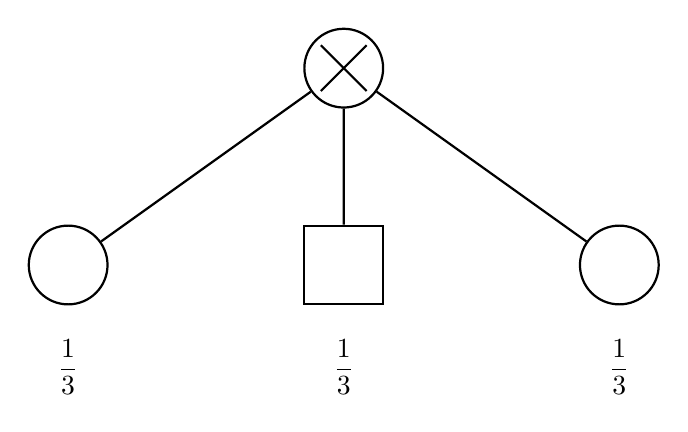
\begin{tikzpicture}[
  thick,
  every node/.style={draw=black, thick},
  level distance=2.5cm,
  level 1/.style={sibling distance=3.5cm},
  edge from parent/.style={draw=black, thick, -},
  grow=down
]

  % Wurzelknoten: Kreis mit X (oben)
  \node[circle, minimum size=1cm] (root) {}
    % Linkes Kind: Kreis
    child {
      node[circle, minimum size=1cm] (left) {}
      edge from parent
    }
    % Mittleres Kind: Rechteck
    child {
      node[rectangle, minimum size=1cm] (mid) {}
      edge from parent
    }
    % Rechtes Kind: Kreis
    child {
      node[circle, minimum size=1cm] (right) {}
      edge from parent
    };

  % X durch die Wurzel zeichnen
  \draw ($(root.north west)!0.1!(root.south east)$)
     -- ($(root.north west)!0.9!(root.south east)$);
  \draw ($(root.north east)!0.1!(root.south west)$)
     -- ($(root.north east)!0.9!(root.south west)$);

  % Brüche unterhalb der Kindknoten
  \node[draw=none, below=0.3cm of left,  font=\sffamily] {$\dfrac{1}{3}$};
  \node[draw=none, below=0.3cm of mid,   font=\sffamily] {$\dfrac{1}{3}$};
  \node[draw=none, below=0.3cm of right, font=\sffamily] {$\dfrac{1}{3}$};

\end{tikzpicture}
\end{document}